\chapter{Latexの環境導入について}
ここまでテンプレートの説明をしてきたが,
まだTeXの環境構築が出来ていないユーザーのために
環境構築の手順を説明する.
作業手順は以下の通りである.
\begin{enumerate}
  \item TeX Liveの導入
  \item VSCodeの導入
  \item latexmkrcの設定
  \item Githubの活用
\end{enumerate}
基本的には\cite{Tex_bilud}を参考としている。

\section{TeXLiveの導入}
ここからインストーラーをダウンロードする。
https://www.tug.org/texlive/acquire-netinstall.html

ページ上のリンク install-tl-windows.exe 
をクリックしてexeファイルをダウンロードする.
install-tl-windows.exeというexeファイルがダウンロードされるので,
実行する.
このとき、セキュリティエラーが出ると思うが無視して実行する.
実行後,図\ref{fig:install_deisplay_1}図\ref{fig:install_deisplay_2}図\ref{fig:install_deisplay_3}までくれば,
インストーラ画面が立ち上がる(\ref{fig:tex_installer}).
\begin{figure}[H]
    \centering
    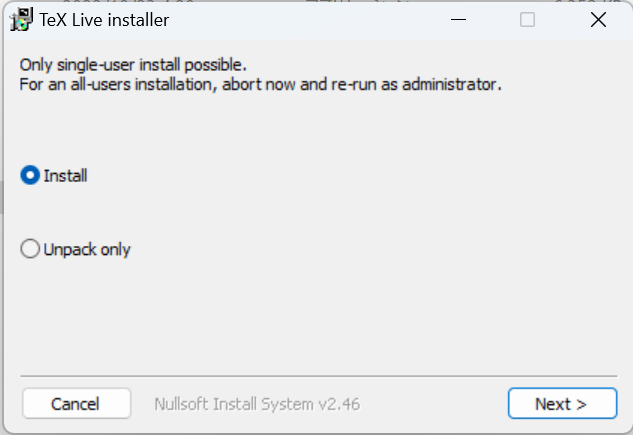
\includegraphics[keepaspectratio, width=0.5\linewidth]{Install_deisplay_1.png}
    \caption{インストール画面1.}
    \label{fig:install_deisplay_1}
\end{figure}

\begin{figure}[H]
  \centering
  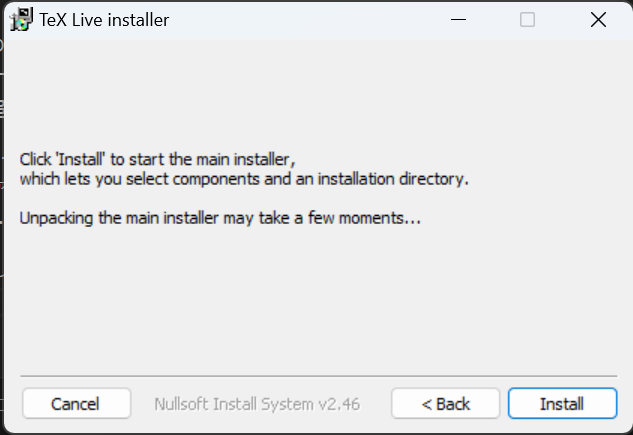
\includegraphics[keepaspectratio, width=0.5\linewidth]{Istall_deisplay_2.png}
  \caption{インストール画面2.}
  \label{fig:install_deisplay_2}
\end{figure}

\begin{figure}[H]
  \centering
  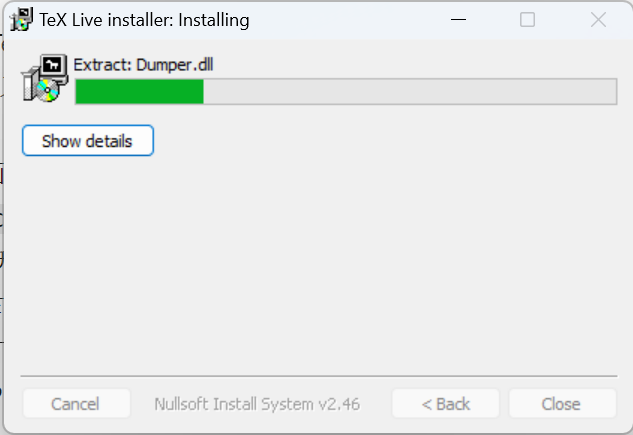
\includegraphics[keepaspectratio, width=0.5\linewidth]{Install_deisplay_3.png}
  \caption{インストール画面3.}
  \label{fig:install_deisplay_3}
\end{figure}

\begin{figure}[H]
  \centering
  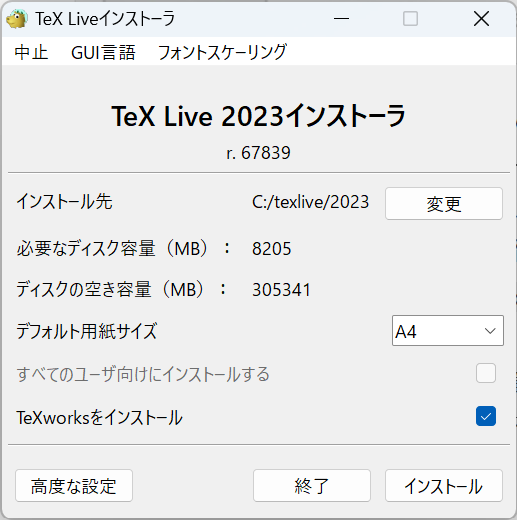
\includegraphics[keepaspectratio, width=0.5\linewidth]{TeX_installer.png}
  \caption{インストーラ画面}
  \label{fig:tex_installer}
\end{figure}

次に「高度な設定」を選択する。
図\ref{fig:installer_setting}が表示される.
ここでは、「ディレクション」,「選択するもの」,「オプション」
の設定を変更できる.
「選択するもの」(図\ref{fig:scheme})
でパッケージを変更する.

\begin{figure}[H]
  \centering
  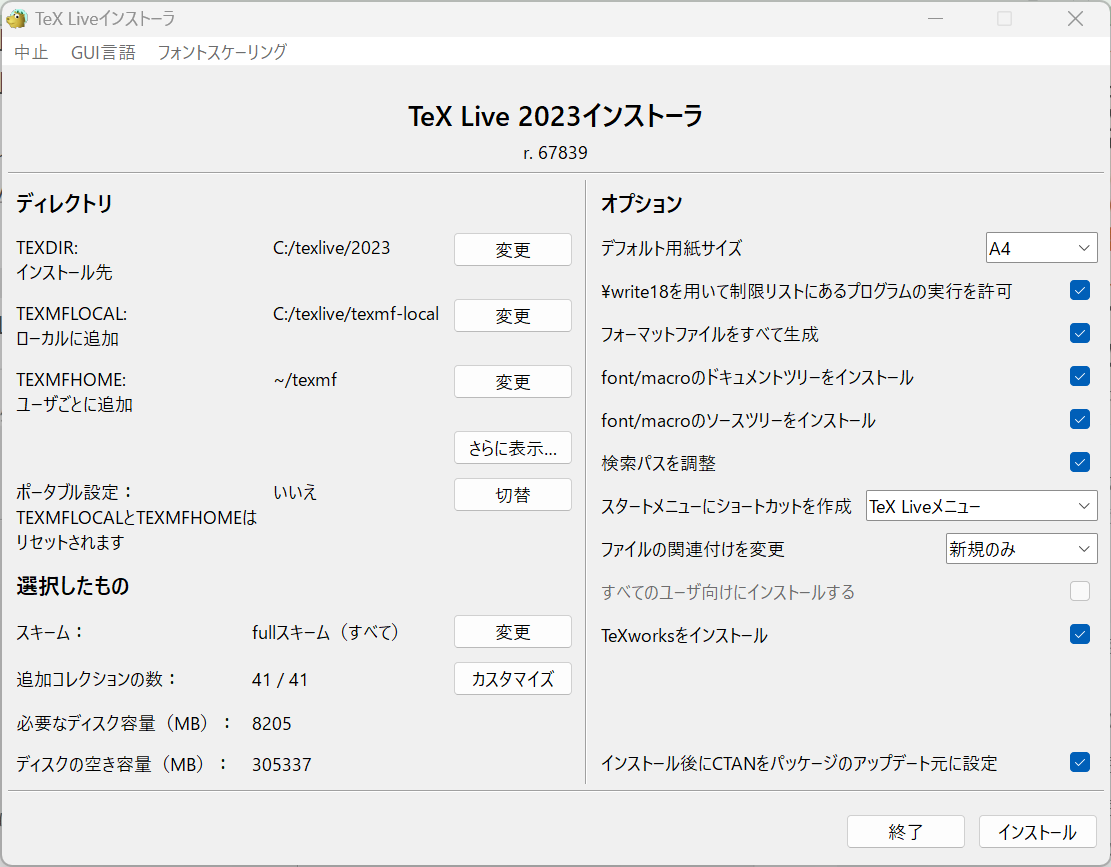
\includegraphics[keepaspectratio, width=0.9\linewidth]{Installer_setting.png}
  \caption{高度な設定画面}
  \label{fig:installer_setting}
\end{figure}

\begin{figure}[H]
  \centering
  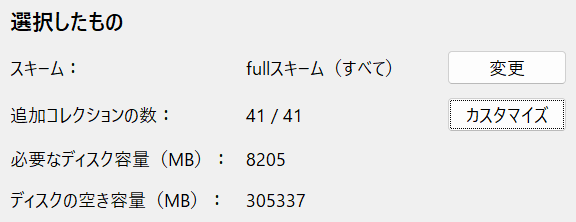
\includegraphics[keepaspectratio, width=0.5\linewidth]{Scheme.png}
  \caption{スキーム選択画面}
  \label{fig:scheme}
\end{figure}

基本的には「fullスキーム」で構わない.
容量が足りない場合には,「plain latex」を選択すれば
最小構成でTexが使える.
スキームの選択が完了したら,「インストール」をクリックする.

\caption{VSCodeの導入}
